\documentclass[11pt,english]{article}
\usepackage[T1]{fontenc}
\usepackage[utf8]{inputenc}
\usepackage[english]{babel}
\usepackage[pdfauthor={Lars Maiwald, Kevin Siebert}]{hyperref}
\usepackage{amsthm}
\usepackage{amssymb}
\usepackage{amsmath}
\usepackage{mathtools}
\usepackage{comment}
\usepackage{pdfpages}
\usepackage{fancyhdr}
\usepackage[headheight=14pt]{geometry}
\usepackage{graphicx}
\usepackage{caption}
\usepackage{subcaption}
\usepackage{siunitx}
\usepackage{csquotes}
\usepackage{hyphenat}
\usepackage{float}
\usepackage{xcolor}
\usepackage{cleveref}
\usepackage{listings}
\usepackage[lighttt]{lmodern}
\usepackage{appendix}
\usepackage{booktabs}
\usepackage[affil-it]{authblk}
\usepackage[backend=biber,style=phys,biblabel=brackets,pageranges=false,sorting=nyt]{biblatex}
\usepackage{multicol}
\usepackage{watermark}
%\addbibresource{}

\lstdefinestyle{CppStyle}{
  language=C++,
  stepnumber=1,
  numbersep=10pt,
  tabsize=4,
  showspaces=false,
  showstringspaces=false
}
\lstdefinestyle{PseudoStyle}{
  basicstyle=\small\ttfamily,
  stepnumber=1,
  numbersep=10pt,
  tabsize=4,
  showspaces=false,
  showstringspaces=false,
  keywordstyle=\color{black}\bfseries\em,
  keywords={,input, output, return, datatype, function, in, if, else, foreach, while, begin, end, }
}
\lstset{basicstyle=\small\ttfamily, style=CppStyle}

\crefname{equation}{}{}
\Crefname{equation}{\text{Equation}}{\text{Equations}}
% \crefname{section}{\text{Kapitel}}{\text{Kapitel}}
% \Crefname{section}{\text{Kapitel}}{\text{Kapitel}}
% \crefname{table}{\text{Tab.}}{\text{Tab.}}
% \Crefname{table}{\text{Tabelle}}{\text{Tabellen}}
% \crefname{figure}{\text{Abb.}}{\text{Abb.}}
% \Crefname{figure}{\text{Abbildung}}{\text{Abbildungen}}

\numberwithin{equation}{section}

%\hyphenation{Mathe-matik wieder-gewinnen}

\sisetup{
locale = DE,
range-phrase = \ldots,
separate-uncertainty=true,
scientific-notation=true,
}

\geometry{
  a4paper,
  left=2.5cm,
  right=2.5cm,
  top=3cm,
  bottom=3cm
}

\renewcommand{\footrulewidth}{0.4pt}
\renewcommand{\headrulewidth}{0.4pt}
\pagestyle{fancy}
\fancyhf{}
\rhead{Maiwald, Siebert}
%\lfoot{}
\lhead{\slshape\nouppercase{\leftmark}}
\cfoot{\thepage}
%\pagestyle{empty}

\hypersetup{
    colorlinks=true,
    linkcolor=blue,
    filecolor=magenta,      
    urlcolor=magenta,
    citecolor=green,
}
\urlstyle{same}

\graphicspath{ {resources/figures/} }

\allowdisplaybreaks

% \setlength\parindent{0pt}

%Einige nützliche Definitionen
\newcommand{\deriv}[2]{\frac{\mathrm{d} #1}{\mathrm{d} #2}}
\newcommand{\pderiv}[2]{\frac{\partial #1}{\partial #2}}
% \newcommand{\kommut}[2]{\left[ #1, #2 \right]}
% \newcommand{\tagthis}[1]{\addtocounter{equation}{1}\tag{\theequation}\label{#1}}
% \newcommand{\tagit}{\addtocounter{equation}{1}\tag{\theequation}}
% \DeclarePairedDelimiter\bra{\langle}{\rvert}
% \DeclarePairedDelimiter\ket{\lvert}{\rangle}
% \DeclarePairedDelimiterX\braket[2]{\langle}{\rangle}{#1 \delimsize\vert #2}
% \DeclarePairedDelimiterX\expval[2]{\langle}{\rangle}{#2 \delimsize\vert #1 \delimsize\vert#2}
% \DeclarePairedDelimiterX\matrixel[3]{\langle}{\rangle}{#1 \delimsize\vert #2 \delimsize\vert#3}
% \DeclarePairedDelimiterX\expv[1]{\langle}{\rangle}{#1}

\newcommand{\ie}{\textit{i.e.} }
\newcommand{\eg}{\textit{e.g.} }

\lstset{
	escapeinside={/*@}{@*/}, language=C++,
	basicstyle=\fontsize{8.5}{12}\selectfont,
	numbers=left,numbersep=2pt,xleftmargin=2pt,frame=tb,
    columns=fullflexible,showstringspaces=false,tabsize=4,
    keepspaces=true,showtabs=false,showspaces=false,
    backgroundcolor=\color{white}, morekeywords={inline,public,
    class,private,protected,struct},captionpos=t,lineskip=-0.4em,
	aboveskip=10pt, extendedchars=true, breaklines=true,
	prebreak = \raisebox{0ex}[0ex][0ex]{\ensuremath{\hookleftarrow}},
	keywordstyle=\color[rgb]{0,0,1},
	commentstyle=\color[rgb]{0.133,0.545,0.133},
	stringstyle=\color[rgb]{0.627,0.126,0.941}
}

\graphicspath{{./resources/images/}}

\thiswatermark{\centering \put(326.5,-68.0){\includegraphics[scale=1.2]{sciences_en.png}}}

\usepackage{abstract}
\newcommand{\myabstract}[1]{
\twocolumn[
  \maketitle             % full width title
  \begin{onecolabstract} % ditto abstract
    {#1}
  \end{onecolabstract}
\vspace{\baselineskip}
]}
\usepackage[backend=biber,style=phys,biblabel=brackets,pageranges=false,sorting=nyt]{biblatex}
\addbibresource{resources/references.bib}

\title{\textbf{Report: \\ Deep learning final project (miniprojects)}}
\author{Kevin Siebert%
	\thanks{\href{mailto:Kevin.Siebert@etu.unige.ch}{Kevin.Siebert@etu.unige.ch}}}
\affil{Department of Informatics, Faculty of Science, \\ University of Geneva}
\date{Dated: \today}

\begin{document}
	\maketitle
	
	\begin{abstract}
		This is a report on the solution of the two mini projects proposed as a final project for the course Deep Learning (14X050). The solutions consists of this report and a GitHub archive containing the corresponding code (\thanks{\href{https://github.com/I-am-Rudi/DL_FinalProject}{Github Archive}})
	\end{abstract}
	
	\section*{Project 1} \label{sec:Introduction}
	\begin{figure}[H]
		\centering
		\includegraphics[width = .75\textwidth]{Simple_network.png}
		\caption{Diagrammatic visualization of the architecture for the simple network. (figure made using Inkscape)}
		\label{fig:sn}
	\end{figure}
	\begin{figure}[H]
		\centering
		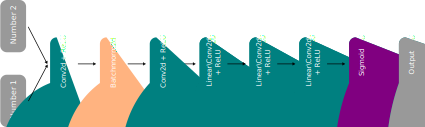
\includegraphics[width = .75\textwidth]{Weight_sharing_network.png}
		\caption{Diagrammatic visualization of the architecture for the weight sharing network.(figure made using Inkscape)}
		\label{fig:ws}
	\end{figure}
	\begin{figure}[H]
		\centering
		\includegraphics[width = .75\textwidth]{Simple_aux_network.png}
		\caption{Diagrammatic visualization of the architecture for the simple auxiliary neural network.(figure made using Inkscape)}
		\label{fig:saux}
	\end{figure}
	\begin{figure}[H]
		\centering
		\includegraphics[width = .75\textwidth]{Classes_aux_network.png}
		\caption{Diagrammatic visualization of the architecture for the auxiliary neural network using the numbers classes. (figure made using Inkscape)}
		\label{fig:caux}
	\end{figure}

	\begin{figure*}
		\centering
		\begin{subfigure}[b]{0.475\textwidth}
			\centering
			\includegraphics[width=\textwidth]{compare/normal-normal/Comparison_Simple_convolutional_network_Weight_sharing_network.png}
			\caption[]%
			{{\small Simple network}}    
		\end{subfigure}
		\hfill
		\begin{subfigure}[b]{0.475\textwidth}  
			\centering 
			\includegraphics[width=\textwidth]{compare/normal-normal/Comparison_Weight_sharing_network_Simple_Auxiliary_classifier_network.png}
			\caption[]%
			{{\small Weight sharing network}} 
		\end{subfigure}
		\vskip\baselineskip
		\begin{subfigure}[b]{0.475\textwidth}   
			\centering 
			\includegraphics[width=\textwidth]{compare/normal-normal/Comparison_Simple_Auxiliary_classifier_network_Auxiliary_classifier_network_using_classes.png}
			\caption[]%
			{{\small Simple auxiliary classifier network}}    
		\end{subfigure}
		\hfill
		\caption[]
		{\small The average and standard deviation of critical parameters: Region R4} 
		\label{fig:comp_normal-normal}
	\end{figure*}

	\begin{figure*}
		\centering
		\begin{subfigure}[b]{0.475\textwidth}
			\centering
			\includegraphics[width=\textwidth]{compare/fc-normal/Comparison_Simple_convolutional_network_Fully_convolutional_network.png}
			\caption[]%
			{{\small Simple network}}    
		\end{subfigure}
		\hfill
		\begin{subfigure}[b]{0.475\textwidth}  
			\centering 
			\includegraphics[width=\textwidth]{compare/fc-normal/Comparison_Weight_sharing_network_Fully_convolutional_weight_sharing_network.png}
			\caption[]%
			{{\small Weight sharing network}} 
		\end{subfigure}
		\vskip\baselineskip
		\begin{subfigure}[b]{0.475\textwidth}   
			\centering 
			\includegraphics[width=\textwidth]{compare/fc-normal/Comparison_Simple_Auxiliary_classifier_network_Fully_convolutional_auxiliary_classifier_network.png}
			\caption[]%
			{{\small Simple auxiliary classifier network}}    
		\end{subfigure}
		\hfill
		\begin{subfigure}[b]{0.475\textwidth}   
			\centering 
			\includegraphics[width=\textwidth]{compare/fc-normal/Comparison_Auxiliary_classifier_network_using_classes_Fully_convolutional_auxiliary_classifier_network_using_classes.png}
			\caption[]%
			{{\small Auxiliary classifier network (number classes)}}    
		\end{subfigure}
		\caption[]
		{\small The average and standard deviation of critical parameters: Region R4} 
		\label{fig:comp_conv-normal}
	\end{figure*}
	
	\begin{figure*}
		\centering
		\begin{subfigure}[b]{0.475\textwidth}
			\centering
			\includegraphics[width=\textwidth]{compare/oh-normal/Comparison_Simple_convolutional_network_Simple_convolutional_network_one_hot_labels=False.png}
			\caption[]%
			{{\small Simple network}}    
		\end{subfigure}
		\hfill
		\begin{subfigure}[b]{0.475\textwidth}  
			\centering 
			\includegraphics[width=\textwidth]{compare/oh-normal/Comparison_Weight_sharing_network_Weight_sharing_network_one_hot_labels=False.png}
			\caption[]%
			{{\small Weight sharing network}} 
		\end{subfigure}
		\vskip\baselineskip
		\begin{subfigure}[b]{0.475\textwidth}   
			\centering 
			\includegraphics[width=\textwidth]{compare/oh-normal/Comparison_Simple_Auxiliary_classifier_network_Simple_Auxiliary_classifier_network_one_hot_labels=False.png}
			\caption[]%
			{{\small Simple auxiliary classifier network}}    
		\end{subfigure}
		\hfill
		\caption[]
		{\small The average and standard deviation of critical parameters: Region R4} 
		\label{fig:comp_conv-oh}
	\end{figure*}

	\begin{figure*}
		\centering
		\begin{subfigure}[b]{0.475\textwidth}
			\centering
			\includegraphics[width=\textwidth]{compare/interesting/Comparison_Simple_convolutional_network_one_hot_labels=False_Weight_sharing_network_one_hot_labels=False.png}
			\caption[]%
			{{\small Simple network}}    
		\end{subfigure}
		\hfill
		\begin{subfigure}[b]{0.475\textwidth}  
			\centering 
			\includegraphics[width=\textwidth]{compare/interesting/Comparison_Weight_sharing_network_one_hot_labels=False_Simple_Auxiliary_classifier_network_one_hot_labels=False.png}
			\caption[]%
			{{\small Weight sharing network}} 
		\end{subfigure}
		\hfill
		\caption[]
		{\small The average and standard deviation of critical parameters: Region R4} 
		\label{fig:comp_int}
	\end{figure*}

	%\printbibliography
\end{document}
